% Asset ID: A22ConditionalProbabilityTikZ-002
% Purpose: Concrete late/not-late conditional tree with changing probabilities.
\documentclass[tikz,border=10pt]{standalone}
\usepackage{amsmath}
\usepackage{tikz}
\usetikzlibrary{arrows.meta, positioning}
\begin{document}
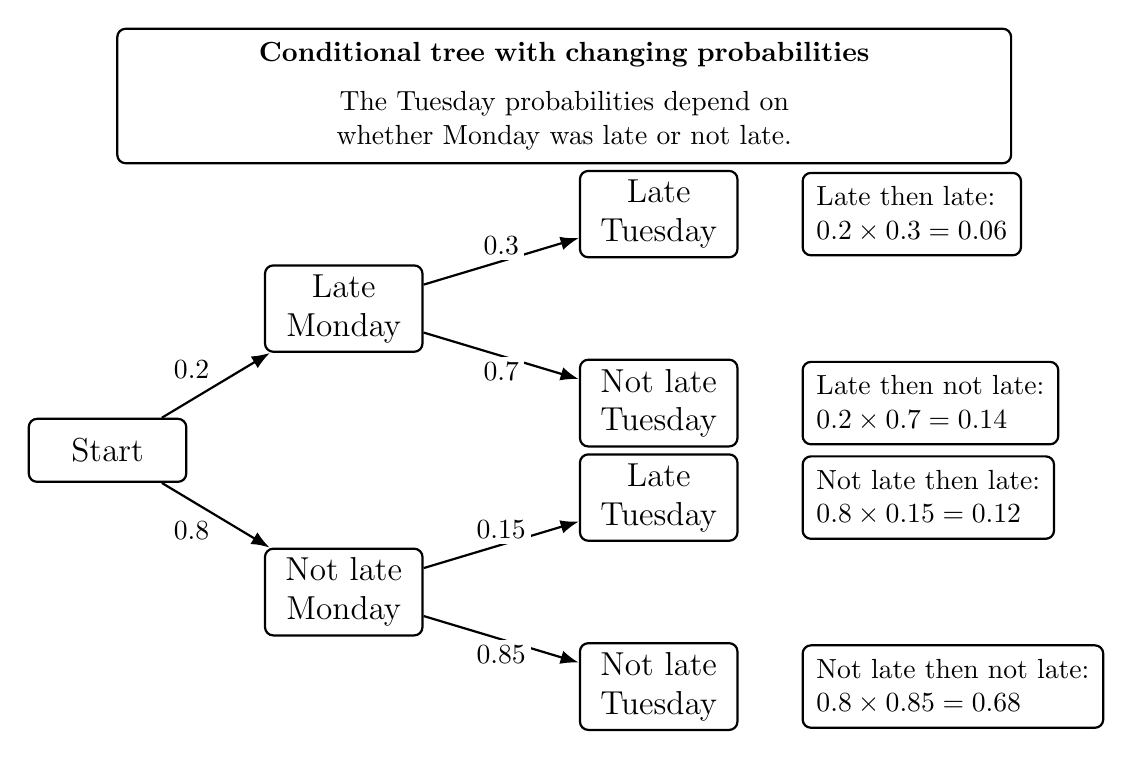
\begin{tikzpicture}[>=Latex,event/.style={rectangle,rounded corners=3pt,draw,thick,minimum width=20mm,minimum height=8mm,font=\large,align=center},note/.style={rectangle,rounded corners=3pt,draw,thick,align=left,inner sep=5pt,font=\normalsize},branchlabel/.style={midway,fill=white,inner sep=2pt,font=\normalsize}]
\node[event] (start) at (0,0) {Start};
\node[event] (Mlate) at (3,1.8) {Late\\Monday};
\node[event] (Mnot) at (3,-1.8) {Not late\\Monday};
\node[event] (TL_LL) at (7,3.0) {Late\\Tuesday};
\node[event] (TN_LL) at (7,0.6) {Not late\\Tuesday};
\node[event] (TL_NL) at (7,-0.6) {Late\\Tuesday};
\node[event] (TN_NL) at (7,-3.0) {Not late\\Tuesday};
\draw[->,thick] (start)--(Mlate) node[branchlabel,above left] {$0.2$};
\draw[->,thick] (start)--(Mnot) node[branchlabel,below left] {$0.8$};
\draw[->,thick] (Mlate)--(TL_LL) node[branchlabel,above] {$0.3$};
\draw[->,thick] (Mlate)--(TN_LL) node[branchlabel,below] {$0.7$};
\draw[->,thick] (Mnot)--(TL_NL) node[branchlabel,above] {$0.15$};
\draw[->,thick] (Mnot)--(TN_NL) node[branchlabel,below] {$0.85$};
\node[note,right=0.8cm of TL_LL] {Late then late:\\$0.2\times0.3=0.06$};
\node[note,right=0.8cm of TN_LL] {Late then not late:\\$0.2\times0.7=0.14$};
\node[note,right=0.8cm of TL_NL] {Not late then late:\\$0.8\times0.15=0.12$};
\node[note,right=0.8cm of TN_NL] {Not late then not late:\\$0.8\times0.85=0.68$};
\node[note,align=center,text width=11cm] at (5.8,4.5) {\textbf{Conditional tree with changing probabilities}\\[2mm]The Tuesday probabilities depend on whether Monday was late or not late.};
\end{tikzpicture}
\end{document}
